\documentclass[10pt,a4paper]{article}
\usepackage[utf8]{inputenc}
\usepackage[frenchb]{babel}
\usepackage{amsmath}
\usepackage{amsfonts}
\usepackage{amssymb}
\usepackage{hyperref}
\usepackage{graphicx}
\author{Bertrand}
\title{Electromagnetique et Méca Flux + rappels mathématiques}

\begin{document} %%% BEGIN DOC

\maketitle
\tableofcontents
\newpage


%%%%%%%%%%%%%%%%%%%%%%%%%%%%%%%%%%%%%%%%%%%%%%%%%%%%%%%%%%%%%%%%%%%%%%%%%
%%%%%%%%%%%%%%%%%%%%%%%%%%%%% RAPPELS MATHEMATIQUES %%%%%%%%%%%%%%%%%%%%%%%%%%%%%
%%%%%%%%%%%%%%%%%%%%%%%%%%%%%%%%%%%%%%%%%%%%%%%%%%%%%%%%%%%%%%%%%%%%%%%%%
\section{Rappels Mathématiques}

%%%%%%%%%%%%% DIVERGENCE %%%%%%%%%%%%%
\subsection{Divergence \cite{divergence}}
\subsubsection{Définition}
La divergence d'un champ de vecteur mesure le défaut de conservation du volume sous l'action du flot de ce champ. Le théorème de flux-divergence \cite{fluxdiv} précise que l'intégrale de la divergence d'un champ de vecteurs sur un volume V définit par une surface fermée S, est égal au flux de ce champ de vecteurs à travers la surface S. Le flux est représenté par un champ de vecteurs et la divergence de ce flux de vecteur représente en chaque point la force de la source ou de la perte en ce point. De manière simplifiée : la somme de tout les gains moins la somme de toutes les pertes est égale au flux. 
\begin{equation}
\iiint_{V}div(\overrightarrow{F})\cdot dV = \iint_{S}\overrightarrow{F}\cdot \overrightarrow{dS}
\end{equation}

$div(\overrightarrow{X})$ est une fonction à valeurs réelles qui mesure la variation première du volume le long des trajectoire dudit champ.
En dimension 3 et en coordonnées cartésiennes pour un champ de vecteurs $\overrightarrow{F}$:
\begin{equation}
div(\overrightarrow{F}) = \overrightarrow{\nabla}\cdot\overrightarrow{F}= \frac{\partial F_{x}}{\partial x} + \frac{\partial F_{y}}{\partial y} + \frac{\partial F_{z}}{\partial z}
\end{equation}

Un champ à divergence nulle est un champ qui conserve le volume, tel que le champ des vecteurs vitesse d'un fluide incompressible.

De manière générale, en physique la divergence est reliée à l'expression locale de la propriété de conservation d'une grandeur. En considérant une surface quelconque S, la variation d'une grandeur conservative dans le volume fermé par cette surface est, par définition une grandeur conservative car il n'existe pas de source de création ou de destruction d'une grandeur conservative. Le bilan de cette grandeur entre deux instants est donc uniquement égale à la somme du flux de cette grandeur à travers la surface S + la variation temporelle de la grandeur à l'intérieur de la surface S. Si cette grandeur est conservative alors le bilan est nul. 

D'où en électromagnétisme par exemple, avec $\overrightarrow{J}$ le vecteur densité de courant et $\rho$ la densité de charges:
\begin{equation}
\iint_{S}\overrightarrow{J}\cdot \overrightarrow{dS} + \frac{d}{dt}\iiint_{V}\rho\cdot dV = 0
\end{equation}


\subsubsection{Propriétés}
Un champ rotationnel est à divergence nulle:
\begin{equation}
div(\overrightarrow{rot}(\overrightarrow{A})) = 0
\label{divrot}
\end{equation}

La divergence peut être vue comme le transposé au signe près, du gradient:
\begin{equation}
div(f\overrightarrow{A}) = f div(\overrightarrow{A}) + \overrightarrow{grad}(f) \cdot \overrightarrow{A}
\end{equation}

- :
\begin{equation}
div(\overrightarrow{A} \land \overrightarrow{B}) = \overrightarrow{B} \cdot \overrightarrow{rot}(\overrightarrow{A}) - \overrightarrow{A} \cdot \overrightarrow{rot}(\overrightarrow{B})
\end{equation}

- :
\begin{equation}
\overrightarrow{rot}(\overrightarrow{rot}(\overrightarrow{A})) = \overrightarrow{grad}(div(\overrightarrow{A})) - \Delta(\overrightarrow{A})
\end{equation}

\subsubsection{Applications}
\paragraph*{Radicaux en carré inverse de la distance}
Le théorème de Gauss nous donne: lorsqu'une loi d'interaction radiale, due à des sources ponctuelles, varie comme le carré inverse de la distance il est possible d'établir que le flux du champ d'interaction à travers une surface fermée est toujours proportionnel à la quantité de sources présentes à l'intérieur de la surface fermée. Par exemple en électromagnétique, avec $Q_{int}$ le nombre de charges dans le volume:
\begin{equation}
\iint_{S}\overrightarrow{E}\cdot\overrightarrow{dS} = \frac{Q_{int}}{\epsilon_{0}}
\end{equation}
Avec le théorème de flux divergence:
\begin{equation}
\iiint_{V}div(\overrightarrow{E})\cdot dV = \frac{Q_{int}}{\epsilon_{0}} = \iiint_{V}\frac{\rho}{\epsilon_{0}}dV
\end{equation}
D'où on en déduit l'équation de Maxwell-Gauss \ref{MaxGauss}. Cette relation est aussi applicable à la gravitation:
\begin{equation}
div(\overrightarrow{G}) = -4\pi G\rho
\end{equation}

\paragraph*{Flux du champ magnétique}
La loi de Maxwell-Thompson \ref{MaxThom} montre que le flux d'un champ magnétique à travers une surface est toujours nul: le champ magnétique est à flux conservatif.
\begin{equation}
\iint_{S}\overrightarrow{B}\cdot \overrightarrow{dS} = \iiint_{V}div(\overrightarrow{B})\cdot dV = 0
\label{consmagn}
\end{equation}


%%%%%%%%%%%%% ROTATIONNEL %%%%%%%%%%%%%
\subsection{Rotationnel \cite{rotationnel}}
\subsubsection{Définition}
L'opérateur rotationnel est un opérateur différentiel aux dérivées partielles qui, à un champ de vecteurs donnés, fait correspondre un autre champ vectoriel.
Il est noté:
\begin{equation}
\overrightarrow{rot}(\overrightarrow{F}) = \overrightarrow{\nabla} \land \overrightarrow{F} = 
\begin{pmatrix}
\frac{\partial F_{z}}{\partial y} - \frac{\partial F_{y}}{z} \\
\frac{\partial F_{x}}{\partial z} - \frac{\partial F_{z}}{x} \\
\frac{\partial F_{y}}{\partial x} - \frac{\partial F_{x}}{y}
\end{pmatrix}
\end{equation}
Le rotationnel exprime la tendance qu'ont les lignes de champs d'un champ vectoriel à tourner autour d'un point: sa circulation locale sur un petit lacet entourant ce point est non nulle quand son rotationnel ne l'est pas. Par exemple:
\begin{description}
\item[Dans une tornade] le vent tourne autour de l'œil du cyclone et le champ vectoriel vitesse du vent a un rotationnel non nul autour de l'œil du cyclone. Plus on se rapproche de l'œil, plus le rotationnel est intense (plus le champ de vorticité/champ tourbillon est intense).
\item[Pour un solide qui tourne a une vitesse $\Omega$] le rotationnel du champ de vitesses et dirigé selon l'axe de rotation, dans le sens direct. La valeur du rotationnel est $2\Omega$.
\end{description}

Le rotationnel d'un champ de vecteurs en un point peut être exprimé comme la circulation locale du champ autour de ce point; cette définition découle du théorème de Green qui donne pour une surface S définie par le contour C:
\begin{equation}
\oint_{C}\overrightarrow{F}\cdot dl = \iint_{S}\overrightarrow{rot}(\overrightarrow{F})\cdot \overrightarrow{dS}
\end{equation}
L'orientation de S et C sont liées tel que $\overrightarrow{dS}\land \overrightarrow{dl}$ est un vecteur dirigé vers la surface (repaire direct).

Le théorème du rotationnel met en relation l'intégrale de volume du rotationnel d'un champ vectoriel avec l'intégrale de surface du même champ. La formule est la suivante, avec S la frontière de V le volume et $\overrightarrow{v}$ le champ vectoriel:
\begin{equation}
\iiint_{V}\overrightarrow{rot}(\overrightarrow{v}) dV = - \iint_{S}\overrightarrow{v}\land \overrightarrow{dS}
\end{equation}

\subsubsection{Propriétés}
Le gradient du rotationel est nul:
\begin{equation}
\overrightarrow{rot}(\overrightarrow{grad}(\overrightarrow{F})) = \overrightarrow{0}
\label{rotgrad}
\end{equation}

La divergence du rotationnel est toujours nulle:
\begin{equation}
div(\overrightarrow{rot}(\overrightarrow{F})) = \overrightarrow{0}
\end{equation}

Le rotationnel du rotationnel est:
\begin{equation}
\overrightarrow{rot}(\overrightarrow{rot}(\overrightarrow{A})) = \overrightarrow{grad}(div(\overrightarrow{A})) - \Delta A
\end{equation}

- :
\begin{equation}
\overrightarrow{rot}(\overrightarrow{A}\cdot\overrightarrow{grad}(\overrightarrow{A})) = \overrightarrow{A}\cdot\overrightarrow{grad}(\overrightarrow{rot}(\overrightarrow{A})) - \overrightarrow{rot}(\overrightarrow{A})\cdot\overrightarrow{grad}(\overrightarrow{A})
\end{equation}


%%%%%%%%%%%%% GRADIENT %%%%%%%%%%%%%
\subsection{Gradient \cite{gradient}}
\subsubsection{Définition}
On définit le gradient comme une grandeur vectorielle qui indique de quelle façon une grandeur physique varie dans l'espace. En mathématiques, le gradient est un vecteur représentant la variation d'une fonction par rapport à ses différents paramètres. En dimension 3:
\begin{equation}
\overrightarrow{grad}(f) = \overrightarrow{\nabla} f = \frac{\partial f}{\partial x}\overrightarrow{x} + \frac{\partial f}{\partial y}\overrightarrow{y} +\frac{\partial f}{\partial z}\overrightarrow{z}
\end{equation}

Construisons le gradient: soit $M$ et $M'$ deux points de l'espace tels que $M$ soit de coordonées $\overrightarrow{u} = (x,y,z)$ et $\overrightarrow{h} = \overrightarrow{MM'} = (h_{x}, h_{y}, h_{z})$. $T$ est une fonction de l'espace. De $M$ à $M'$, $T$ passe de $T(x,y,z)$ à $T(x+h_{x}, y+h_{y}, z+h_{z})$. En première approximation, cette variation est une fonction linéaire de $\overrightarrow{h}$ :
\begin{equation}
T(x+h_{x}, y+h_{y}, z+h_{z}) = T(x,y,z) + \frac{\partial T}{\partial x}(x,y,z)h_{x}  + \frac{\partial T}{\partial y}(x,y,z)h_{y} + \frac{\partial T}{\partial z}(x,y,z)h_{z}
\label{graddl1}
\end{equation}
On créer alors le vecteur appelé gradient de température:
\begin{equation}
\overrightarrow{grad}(T(x,y,z)) = 
\begin{pmatrix}
\frac{\partial T}{\partial x}(x,y,z) & \frac{\partial T}{\partial y}(x,y,z) & \frac{\partial T}{\partial z}(x,y,z)
\end{pmatrix}
\end{equation}
Et on peut écrire la relation \ref{graddl1} sous la forme d'un développement linéaire:
\begin{equation}
T(\overrightarrow{u} + \overrightarrow{h}) = T(\overrightarrow{u}) + \overrightarrow{grad}(T(\overrightarrow{u}))\cdot\overrightarrow{h} + o(\overrightarrow{h})
\end{equation}
Où $o(\overrightarrow{h}$ signifie que le terme qui reste est négligeable devant $\overrightarrow{h}$.

\subsubsection{Propriétés}
EN dimension 2, le gradient normal à une courbe en un point est la droite tangente.

En dimension 3, le gradient normal à une surface en un point est le plan tangent.

Gradient et convexité: Soit une application $f: \Re^{n} \mapsto \Re$ où $n \in \{2,3\}$ par exemple, continuement dérivable. Si l'application $\overrightarrow{grad}(f): \Re^{n} \mapsto \Re^{n}$ est monotomne (resp. strictement monotone) alors $f$ est convexe (resp. strictement convexe). C'est à dire en caractérisant par les cordes:
\begin{equation}
\forall (u,v) \in (\Re^{3})^2, \overrightarrow{grad}_{u}(f)\cdot\overrightarrow{grad}_{v}(f) \geq 0 
\implies
\forall (u,v,\lambda) \in \Re^{3} \times \Re^{3} \times [0,1], f(\lambda u + (1-\lambda)v) \leq \lambda f(u)+(1-\lambda)f(v)
\label{gradconv}
\end{equation}
La propriété \ref{gradconv} est valable même si $f$ n'est pas deux fois dérivable.

D'autres relations vectorielles:
\begin{equation}
\frac{\partial}{\partial t}\overrightarrow{grad}(f) = \overrightarrow{grad}(\frac{\partial f}{\partial t})
\end{equation}
\begin{equation}
div(\overrightarrow{grad}(f)) = \Delta f
\end{equation}
\begin{equation}
\overrightarrow{rot}(\overrightarrow{grad}(f)) = \overrightarrow{0}
\end{equation}


%%%%%%%%%%%%% EQUATION DE LAPLACE %%%%%%%%%%%%%
\subsection{Équation de Laplace \cite{eqlaplace}}
\subsubsection{Définition}
En coordonnées cartésiennes dans un espace euclidine de dimension 3, le problème consiste à trouver lles fonctions $f(x,y,z)$ qui vérifient:
\begin{equation}
\frac{\partial^{2} f}{\partial x^{2}} + \frac{\partial^{2} f}{\partial y^{2}} + \frac{\partial^{2} f}{\partial z^{2}} = 0
\end{equation}
On introduit alors l'opérateur Laplacien noté $\Delta$, et l'équation devient:
\begin{equation}
\Delta f = 0
\end{equation}
L'opérateur peut aussi être noté $\nabla^{2}$ et il est aussi égal à $div(\overrightarrow{grad}(f))$.

\subsubsection{Fontions harmoniques \cite{fharmonique}}
Les fonctions harmoniques sont définies comme étant des fonctions deux fois continument dérivables et solution de l'équation de Laplace. Soit $U$ un ouvert de $\Re^{n}$. Une application $f : U \mapsto \Re$ est dite harmonique si:
\begin{equation}
\frac{\partial^{2} f}{\partial x_{1}^{2}} + \frac{\partial^{2} f}{\partial x_{2}^{2}} + \dotsb + \frac{\partial^{2} f}{\partial x_{n}^{2}} = 0
\end{equation}

\subsubsection{Résultats}
En étudiant les solutions de l'équation, on prouve que:
\begin{itemize}
\item Toute fonction holomorphe\cite{fholomorphe} est harmonique.
\item Les lignes de niveaux\cite{ligneniveau} de la partie réelle et imaginaire d'une fonction holomorphe sont orthogonales.
\end{itemize}




%%%%%%%%%%%%%%%%%%%%%%%%%%%%%%%%%%%%%%%%%%%%%%%%%%%%%%%%%%%%%%%%%%%%%%%%%%%%%%%%%%%
%%%%%%%%%%%%%%%%%%%%%%%%%%%%%%%%%%% ELECTROMAGNETIQUE %%%%%%%%%%%%%%%%%%%%%%%%%%%%%%%%%%%
%%%%%%%%%%%%%%%%%%%%%%%%%%%%%%%%%%%%%%%%%%%%%%%%%%%%%%%%%%%%%%%%%%%%%%%%%%%%%%%%%%%
\section{Électromagnétique}
\subsection{Rappels électromagnétique}

%%%%%%%%%%%%% DENSITE DE COURANT %%%%%%%%%%%%%
\subsubsection{Densité de courant \cite{denscour}}
Elle décrit le courant électrique qui circule à l'échelle locale (en un point du matériau). Il s'agit d'un champ de vecteurs qui associe à tout point de l'espace un vecteur densité de courant. Son unité est : $A.m^{-2}$. Le courant électrique est le débit de charges électriques à travers une surface orienté $\overrightarrow{dS}$.
\begin{equation}
di = \overrightarrow{j}\cdot\overrightarrow{dS} \implies i = \iint_{S}\overrightarrow{j}\cdot\overrightarrow{dS}
\label{densCour}
\end{equation}
Dans la formule \ref{densCour}, le signe de i est lié à l'orientation de $\overrightarrow{dS}$.
Lorsqu'une des dimensions est très petite devant les autres (ex: plaque), on peut alors définir la densité de courant surfacique.

%%%%%%%%%%%%% PERMITTIVITE DIELECTRIQUE %%%%%%%%%%%%%
\subsubsection{Permittivité diélectrique \cite{permelec}}
Elle décrit la réponse d'un milieu à un champ électrique. Au niveau microscopique, elle est liée à la polarisabilité électrique des molécules ou atomes du matériau. Son unité est: Coulombs ou F/m.
La valeur le permittivité diélectrique du vide est:
\begin{equation}
\epsilon_{0} = 8,854187.10^{-2} F\cdot m^{-1}
\end{equation}

On définit la permittivité relative d'un matériau par rapport à celle du vide. Avec $\epsilon_{r}$ permittivité relative(sans unité), $\epsilon$ permittivité du milieu, $\epsilon_{0}$ permittivité du vide:
\begin{equation}
\epsilon_{r} = \frac{\epsilon}{\epsilon_{0}}
\end{equation}
$\epsilon$ est généralement complexe: la partie imaginaire étant liée à l'absorption/émission de champ électromagnétique. La partie réelle et imaginaire sont liées par les relations de Kramers-Kronig.

Dans le très simple cas d'un matériau linéaire, homogène, isotrope, et avec réponse instantanée aux changements du champ électrique, la relation des champs électrique et d’induction à la permittivité est :
\begin{equation}
\overrightarrow{D} = \epsilon \overrightarrow{E}
\label{InducPermElec}
\end{equation}

Dans les milieux plus complexe:
\begin{itemize}
\item Si le matériau n'est pas isotrope, $\epsilon$ est une matrice et $\overrightarrow{D}$ n'est plus colinéaire à $\overrightarrow{E}$.
\item Si le matériau n'est pas homogène, les coefficients $\epsilon_{i,j}$ de la matrice dépendent des coordonnées dans l'espace.
\item Si le matériau n'est pas à réponse instantanée, les coefficients de la matrice dépendent des coordonnées de temps et/ou de fréquence.
\item Si le matériau n'est pas linéaire, la relation \ref{InducPermElec} n'est plus valable.
\end{itemize}


%%%%%%%%%%%%% PERMEABILITE MAGNETIQUE %%%%%%%%%%%%%
\subsubsection{Perméabilité magnétique \cite{permmag}}
En régime linéaire, elle caractérise la faculté d'un matériau à modifier un champ magnétique, i.e modifier les lignes de flux magnétique. Son unité est: $M\cdot m^{-1}$.
La valeur de la perméabilité magnétique du vide ou constante  magnétique est:
\begin{equation}
\mu_{0} = 4\pi 10^{-7} H.m^{-1}
\end{equation}

 Dans le cas d'un régime linéaire, le champ d'excitation magnétique et le champ magnétique sont reliés par la relation:
\begin{equation}
\overrightarrow{B} = \mu\cdot \overrightarrow{H}
\end{equation}

On distingue 3 types de matériaux: dia-magnétiques, paramagnétiques, ferromagnétiques. La perméabilité des matériaux dia-magnétiques et paramagnétiques est très proche de celle du vide. La perméabilité des matériaux ferromagnétiques dépend de l'excitation magnétique $\overrightarrow{H}$. De manière générale, la canalisation du champ magnétique dans un matériaux qui est aussi conducteur est d'autant plus réduite que la fréquence de variation des champs, la perméabilité et la conductivité sont élevées.



%%%%%%%%%%%%%%%%%%%%%%%%%%%%%%%%%%%%%%%%%%%%%%%%%%%%%%%%%%%%%%%%%%%%%%%%%%%%%%%%%%%%%%%%
\subsection{Équations de Maxwell}
%%%%%%%%%%%%% MAXWELL GAUSS %%%%%%%%%%%%%
\subsubsection{Maxwell-Gauss}
\begin{equation}
div(\overrightarrow{E}) = \frac{\rho}{\epsilon_{0}}
\label{MaxGauss}
\end{equation}
Donne la divergence du champ électrique en fonction de la densité des charges. C'est une équation de "terme source": la densité de charges électriques est une source de champ électrique.
On peut déduire de la formule \ref{MaxGauss}, le champ électrostatique en un point M, créé par une charge ponctuelle q au point O. En notant $\overrightarrow{OM} = r\cdot\overrightarrow{u_{r}}$, on obtient:
\begin{equation}
\overrightarrow{E}(M) = \frac{q}{4\pi\epsilon_{0}r^{2}}\cdot\overrightarrow{u_{r}}
\end{equation}

%%%%%%%%%%%%% MAXWELL THOMSON %%%%%%%%%%%%%
\subsubsection{Maxwell-Thompson}
\begin{equation}
div(\overrightarrow{B}) = 0
\label{MaxThom}
\end{equation}
Cette équation est l'équivalente locale pour le champ magnétique, de l'équation \ref{MaxGauss}, de Maxwell-Gauss, i.e équation avec "terme de source". Le champ magnétique est à flux conservatif, cf \ref{consmagn}. On en déduit aussi qu'il n'existe pas de monopole magnétique: quand on coupe un aimant en deux, on n'obtient pas 1 pôle sud et un pôle nord mais deux nouveaux aimants.

En prenant la réciproque l'équation \ref{divrot}, du divergent, tout champ de vecteurs dont la divergence est nulle peut-être exprimé sous forme de rotationnel. On peut donc définir le potentiel vecteur $\overrightarrow{A}$, tel que:
\begin{equation}
\overrightarrow{B} = \overrightarrow{rot}(\overrightarrow{A})
\end{equation}

%%%%%%%%%%%%% MAXWELL FARADAY %%%%%%%%%%%%%
\subsubsection{Maxwell-Faraday}
\begin{equation}
\overrightarrow{rot}(\overrightarrow{E}) = - \frac{\partial\overrightarrow{B}}{\partial t}
\label{MaxFar}
\end{equation}
Donne la dérivée temporelle du champ magnétique en fonction du champ électrique. Cette équation correspond à un terme variationnel: la variation du champ magnétique crée un champ électrique. L'expression sous sa forme intégrale donne:
\begin{equation}
\oint_{C}\overrightarrow{E}\cdot\overrightarrow{dl} = - \int_{S}\frac{\partial\overrightarrow{B}}{\partial t}\cdot\overrightarrow{dS}
\end{equation}
En prenant la réciproque à l'équation \ref{rotgrad}, du rotationnel,  tout champ de vecteurs dont le rotationnel est nul peut être écrit sous la forme d'un gradient, puis en factorisant la dérivée par rapport à t, on définit un potentiel scalaire électrique V tel que:
\begin{equation}
\overrightarrow{E} = - \overrightarrow{grad}(V) - \frac{\partial\overrightarrow{A}}{\partial t}
\end{equation}
Pour rappel la loi de Faraday qui donne la force électromotrice $\epsilon$ en fonction du flux magnétique $\Phi$ est:
\begin{equation}
\epsilon = - \frac{d\Phi}{dt}
\end{equation}

%%%%%%%%%%%%% MAXWELL AMPERE %%%%%%%%%%%%%
\subsubsection{Maxwell-Ampère}
\begin{equation}
\overrightarrow{rot}(\overrightarrow{B}) = \mu_{0}\overrightarrow{j} + \mu_{0}\epsilon_{0}\frac{\partial\overrightarrow{E}}{\partial t}
\label{MaxAmp}
\end{equation}
Cette formule introduit la densité de courant :$\overrightarrow{j}$.
Sous sa forme intégrale la formule \ref{MaxAmp} lie la circulation sur un contour fermé C et les courants qui traversent une surface S s'appuyant sur ce même contour C:
\begin{equation}
\oint_{C}\overrightarrow{B}\cdot\overrightarrow{dl} = \mu_{0}\iint_{S}\overrightarrow{j}\cdot\overrightarrow{dS} + \mu_{0}\epsilon_{0}\iint_{S}\frac{\partial\overrightarrow{E}}{\partial t}\cdot\overrightarrow{dS}
\end{equation}
En appliquant l'opérateur divergence à la formule \ref{MaxAmp}, on obtient:
\begin{equation}
div(\overrightarrow{j}) + \frac{\partial \rho}{\partial t} = 0
\end{equation}


%%%%%%%%%%%%%%%%%%%%%%%%%%%%%%%%%%%%%%%%%%%%%%%%%%%%%%%%%%%%%%%%%%%%%%%%%%%%%%%%%%%
%%%%%%%%%%%%%%%%%%%%%%%%%%%%%%%%%%%%%% ANTENNES %%%%%%%%%%%%%%%%%%%%%%%%%%%%%%%%%%%%%%
%%%%%%%%%%%%%%%%%%%%%%%%%%%%%%%%%%%%%%%%%%%%%%%%%%%%%%%%%%%%%%%%%%%%%%%%%%%%%%%%%%%
\section{Antennes}
A FAIRE



%%%%%%%%%%%%%%%%%%%%%%%%%%%%%%%%%%%%%%%%%%%%%%%%%%%%%%%%%%%%%%%%%%%%%%%%%%
%%%%%%%%%%%%%%%%%%%%%%%%%%%%%  MECANIQUE DES FLUIDES  %%%%%%%%%%%%%%%%%%%%%%%%%%%%%
%%%%%%%%%%%%%%%%%%%%%%%%%%%%%%%%%%%%%%%%%%%%%%%%%%%%%%%%%%%%%%%%%%%%%%%%%%
\section{Mécanique des fluides}
La mécanique des fluides est une branche de la mécanique des milieux continus qui étudie le comportement des fluides et de leurs forces internes. Elle considère des particules assez petites pour l'analyse mathématique mais plus grande que les molécules pour être décrites comme des fonctions continues, on dit que l'on considère les fluides comme étant continus. Aujourd'hui il y a encore de nombreux problèmes non résolus comme l'étude des turbulences. La recherche utilise systématiquement des outils numériques regroupés sous le terme "Computational fluid dynamics".

\subsection{Propriétés des fluides}

%%%%%%%%%%%%%  PRESENTATION DU PROBLEME  %%%%%%%%%%%%%
\subsubsection{Présentation du problème \cite{intromecaflu}}
La viscosité d'un fluide est décrite par son nombre de Reynolds\cite{nbreynolds}. Tous les fluides sont visqueux: le mouvement d'une couche de fluide par rapport à une autre est freinée par des phénomènes de frottement. Pour un fluide Newtonien, la force tangentielle est proportionnelle au taux de variation de la vitesse: ce qui conduit aux équations de Navier-Strokes.

Pour un fluide visqueux s'écoulant contre une paroi, la vitesse de la couche de fluide contre la paroi est nulle. Lorsque la viscosité est importante (nombre de Reynolds $<$ 1) l'écoulement est laminaire, c'est l'écoulement de Strokes. En s'éloignant assez des parois les vitesses deviennent quasi-constantes ce qui permet de négliger la viscosité, plus le nombre de Reynolds est élevé dans cette zone plus on peut considérer le fluide comme parfait et ainsi appliquer les équations d'Euler.

Cependant pour dans une première gamme de nombre de Reynolds l'écoulement reste irrotationnel (pas de tourbillons). Pour de plus fortes valeur de nombre de Reynolds, la couche limite engendre un sillage tourbillonnaire (avec rotationnel). Pour des valeurs encore plus élevée du nombre de Reynolds, la couche limite est laminaire en amont mais turbulente en aval.

Il faut aussi considérer la compressibilité du fluide, décrite par le nombre de Mach\cite{nbmach}.

Dans un fluide on observe différents régimes d'écoulement. 

Mathématiquement on distingue les régimes:
\begin{description}
\item[permanents (ou stationnaires)] les grandeurs ne dépendent pas du temps.
\item[uniformes] la vitesse ne dépend pas du point considéré.
\end{description}

Physiquement on distingue les régimes:
\begin{description}
\item[laminaires] les couches de fluides glissent les unes par rapport aux autres, les vitesses sont continues.
\item[turbulents] les vitesses sont discontinues, les couches de fluides s'interpénètrent de manière aléatoire.
\item[tourbillonnaires] qui apparait fréquemment dans la transition laminaire-turbulent.
\end{description}

%%%%%%%%%%%%% FLUIDE COMPRESSIBLE ET INCOMPRESSIBLE %%%%%%%%%%%%%
\subsubsection{Fluide compressible et incompressible}
Si les changement de densité d'un fluide ont des effets significatif sur les résultats, on dit que le fluide est compressible. Dans le cas contraire le fluide est incompressible et les changements de densité sont ignorés.

Le nombre de Mach\cite{nbmach} permet de déterminer la compressibilité d'un fluide. On considère un fluide comme compressible pour des nombre de Mach supérieurs à $0.3$.

Explication de la compressibilité: en acoustique, l'air doit être considéré comme un fluide compressible sinon la propagation du son dans l'air serait instantanée (vitesse infinie). Pour note, la vitesse de propagation du son\cite{vitesseson} dans un \textbf{liquide} de coefficient de compressibilité adiabatique $\chi$ est:
\begin{equation}
c^{2} = (\rho_{0}\chi)^{-1}
\end{equation}

%%%%%%%%%%%%%  VISCOSITE  %%%%%%%%%%%%%
\subsubsection{Viscosité}
Dans les problèmes où les frottements entre les couches de fluides ont des effets non négligeables sur la solution, les fluides sont considérés visqueux. Sinon ils sont appelés non-visqueux. 

Le nombre de Reynolds\cite{nbreynolds} est employé pour estimer quel type d'équations doit être utiliser pour résoudre un problème: pour des écoulements à faible nombre de Reynolds (près d'une paroi) l'écoulement est laminaire, on utilisera les équations de Navier-Strokes. Pour des nombres de Reynolds élevés, l'écoulement pourra être considéré comme non-visqueux (donc non laminaire) et les équations d'Euler seront utilisée.

\textbf{ATTENTION}: il arrive que même si le nombre de Reynolds est élevé, il faille considérer les effets de viscosité, par exemple pour un écoulement autour d'une aile d'avion (cf paradoxe de D'Alembert\cite{paradoxealembert}).

%%%%%%%%%%%%%  ECOULEMENT STATIONNAIRE ET INSTATIONNAIRE %%%%%%%%%%%%%
\subsubsection{Écoulement stationnaire et instationnaire}
Le fluide est considéré comme stationnaire si toutes ses propriétés sont considérées comme constantes avec le temps. Ceci constitue une bonne approximation pour des problèmes tels que la trainée d'une aile, la poussée ou un fluide traversant un tuyau. Dans ce cas les équations de Navier-Strokes peuvent être simplifiées.

Si un fluide est incompressible, non-visqueux et stationnaire il peut être résolu avec l'écoulement potentiel découlant de l'équation de Laplace.

%%%%%%%%%%%%%  ECOULEMENT LAMINAIRE ET TURBULENCES %%%%%%%%%%%%%
\subsubsection{Écoulement laminaire et turbulences}
La turbulence est un écoulement avec remous et un aspect aléatoire apparent. S'il n'y a pas de turbulences, l'écoulement est laminaire. Les turbulences obéissent à l'équation de Navier-Strokes, cependant la résolution est si complexe qu'il n'est pas possible actuellement de les résoudre numériquement avec les principes de base. Les turbulences sont plutôt modélisées avec un des nombreux modèles de turbulence couplée avec un résolveur de flux laminaires.



%%%%%%%%%%%%%%%%%%%%%%%%%%%%%%%%%%%%%%%%%%%%%%%%%%%%%%%%%%%%%%%%%%%%%%%%%%%%%%%%%%%%%%%%
\subsection{Formules de mécanique des fluides}
%%%%%%%%%%%%%  NOMBRE RE REYNOLDS %%%%%%%%%%%%%
\subsubsection{Nombre de Reynolds\cite{nbreynolds}}
Le nombre de Reynolds est sans dimension. Il caractérise un écoulement: sa nature et son régime (laminaire, transitoire, turbulent ...). Il représente le rapport entre les forces d'intertie et les forces visqueuses. Il est définit tel que:
\begin{equation}
Re = \frac{VL}{\upsilon}
\end{equation}
Avec $V$ vitesse caractéristique du fluide ($m.s^{-1}$), $L$ dimension caractéristique ($m$), $\upsilon$ viscosité cinématique $(m^{2}.s^{-1})$.

%%%%%%%%%%%%% VISCOSITE CINEMATIQUE  %%%%%%%%%%%%%
\subsubsection{Viscosité cinématique\cite{viscocinema}}
La viscosité cinématique représente la capacité de rétention des particules du fluide et quantifie sa capacité à s'épancher. Elle est reliée à la viscosité dynamique par:
\begin{equation}
\upsilon = \frac{\mu}{\rho}
\end{equation}
Où $\upsilon$ est la viscosité cinématique ($m^{2}.s^{-1}$), $\mu$ le coefficient de viscosité dynamique ($Pa.s$), $\rho$ la masse volumique du fluide ($kg.m^{-3}$).

%%%%%%%%%%%%% VISCOSITE DYNAMIQUE  %%%%%%%%%%%%%
\subsubsection{Viscosité dynamique\cite{viscodyna,viscodyna2,viscodyna3}}
La viscosité est une mesure des fictions internes d'un fluide, qui apparait lorsqu'une tranche de fluide doit se déplacer par rapport à une autre. La figure \ref{fig:viscodyna} montre le modèle utilisé par Newton. Deux plans parallèles de fluides de surfaces égales $S$ sont séparés par une distance $dx$ et se déplacent dans la même direction à des vitesses $V$ et $V+dv$. Newton à supposé que la force nécessaire pour maintenir cette différence de vitesse était proportionnelle au gradient de vitesse. C'est à dire:
\begin{equation}
\frac{F}{S} = -\mu \frac{dv}{dx}
\end{equation}
Où $\mu$ est une constante pour un fluide donné, et appelé coefficient de viscosité dynamique. Le gradient de vitesse $\frac{dv}{dx}$ est une mesure de la variation de vitesse à laquelle les couches du fluides se déplacent l'une par rapport à l'autre; il décrit le cisaillement que subit le liquide, il est ainsi appelé taux de cisaillement. Le terme $\frac{F}{S}$ est appelé contrainte de cisaillement. Ainsi on peut définir le coefficient de viscosité dynamique comme le rapport de contrainte de cisaillement sur le taux de cisaillement.

Pour développer son modèle Newton avait supposé que pour une température donnée, le coefficient de viscosité dynamique était indépendant du gradient de vitesse, i.e si on double la force le fluide se déplacera deux fois plus vite. Au vu des expérience, ce n'est que partiellement vrais. On distingue ainsi deux types de fluides:
\begin{description}
\item[Les fluides newtoniens] dont le coefficient de viscosité dynamique est indépendant du gradient de vitesse. C'est le cas des gaz, vapeurs, liquides purs de faible masse molaire
\item[Les fluides non-newtoniens] dont le coefficient de viscosité dynamique dépend du gradient de vitesse. L'étude de ce type de fluides dépend de la rhéologie. Ces fluides sont beaucoup plus communs: purées, gels, sang, boues, peintures, solutions de polymères, ...
\end{description}

\begin{figure}
\centering
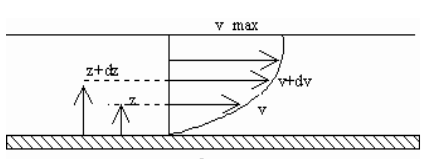
\includegraphics[scale=0.5]{viscodyna}
\caption{Modèle de la viscosité}
\label{fig:viscodyna}
\end{figure}

Le coefficient de viscosité correspond au coefficient de diffusion de la quantité de mouvement. C'est grâce à la viscosité que le mouvement d'une couche de fluide peut induire et transmettre des mouvements dans les couches voisines.

%%%%%%%%%%%%% NOMBRE DE MACH  %%%%%%%%%%%%%
\subsubsection{Nombre de Mach\cite{nbmach}}
C'est un nombre sans dimensions, qui exprime le rapport de la vitesse locale d'un fluide à la vitesse du son dans ce même fluide. Les propriétés d'un fluide variant avec sa nature et sa température, le nombre e de Mach ne correspond pas à une vitesse fixe, il dépend des conditions locales. Il mesure le rapport entre les forces liées au mouvement et la compressibilité du fluide:
\begin{equation}
Ma = \frac{U}{a}
\end{equation}
Où $Ma$ est le nombre de Mach, $U$ est la vitesse de l'objet par rapport à son environnement et $a$ la vitesse de propagation du son\cite{vitesseson} dans l'environnement considéré. Le nombre de mach caractérise différent types d'écoulements:
\begin{itemize}
\item $Ma < 0,94$ : on parle d'écoulement subsonique.
\item $ 0,94 < Ma < 1,2$ : on parle d'écoulement transsonique.
\item $1,2 < Ma < 5$ : on parle d'écoulement supersonique.
\item $Ma > 5$ : on parle d'écoulement hypersonique.
\end{itemize}


Étudions l'exemple d'un objet volant (cf. figure\ref{fig:ecoulementmach}):
\begin{figure}
\centering
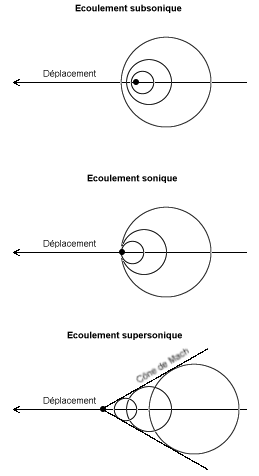
\includegraphics[scale=0.5]{ecoulementmach}
\caption{Différents écoulement en fonction du nombre de Mach}
\label{fig:ecoulementmach}
\end{figure}
\begin{description}
\item[Écoulement subsonique, $Ma<1$] l'objet, qui a une vitesse inférieure à celle de l'accroissement des sphères de perturbation qu'il crée à chaque instant, se trouve en permanence à l'intérieur de celles-ci. Ce déplacement donne également naissance à l'effet Doppler\cite{effetdoppler}.
\item[Écoulement sonique, $Ma=1$] l'objet colle en permanence à l'avant de toutes les sphères de perturbation, qui se retrouvent toutes tangentes à un plan perpendiculaire au mouvement de l'objet. Cet superposition de petites perturbation augmente considérablement la résistance de l'air: c'est le mur du son.
\item[Écoulement supersonique, $Ma>1$] l'objet laisse au contraire toutes les sphères de perturbation derrière lui. Un raisonnement simple montre qu'elles sont toutes tangentes à un cône appelé cône de Mach.
\end{description}

%%%%%%%%%%%%% DESCRIPTION LAGRANGIENNE ET EULERIENNE  %%%%%%%%%%%%%
\subsubsection{Description Lagrangienne vs Description Eulérienne}
La dynamique des fluides dispose de deux techniques d'études: l'approche Lagrangienne et l'approche Eulérienne.

\paragraph{La description Eulérienne\cite{desceuler}} définie à tout instant une valeur pour chaque point de l'espace; en mécanique des fluide c'est généralement un champ de vecteurs vitesses. Le champ de vitesse $V$ donne en tout instant et position le vecteur vitesse associé: $V(M, t)$. Si cette fonction vectorielle ne dépend pas de $t$, l'écoulement et stationnaire. Cette représentation est généralement préférée à l'approche Lagrangienne. La variation de vitesse au cours du temps est alors décrite par la dérivée partielle, encore appelée dérivée Eulérienne.

\paragraph{La description Lagrangienne\cite{desclagrange}} au contraire, suit chacune des particule de fluide dans le temps, le long de leurs trajectoires respectives. Dans ce modèle, la position $M$ d'une particule se trouvant à l'instant $t$ à la position $M_{0}$ est donnée par une relation du type: $M = f(M_{0}, t)$. Avec cette méthode, le référentiel se déplace avec le fluide, il est donc difficile de connaitre l'état du fluide en un point donné de l'espace et du temps. Une variation est définie par la dérivée particulaire, ou totale, ou encore Lagrangienne qui tiens compte de la variation locale du paramètre au cours du temps mais aussi de la variation de celui-ci lié au déplacement de la particule.

\paragraph{Pour passer d'une représentation à l'autre} on utilise la dérivée particulaire. Trouvons la relation entre la dérivé Lagrangienne et la dérivée Eulérienne pour un mouvement à une dimension pour une particule située en $x$ se déplaçant à la vitesse $v$. Un développement limité à l'ordre 1 donne:
\begin{equation}
df = f(x+vdt, t+dt) - f(x, t) = \frac{\partial f}{\partial x} vdt + \frac{\partial f}{\partial t} dt
\end{equation}
En divisant par $dt$ on obtient la notation conventionnelle:\begin{equation}
\frac{Df}{Dt} = \frac{\partial f}{\partial t} + v \frac{\partial f}{\partial x}
\end{equation}
En généralisant à plusieurs dimensions on obtient:
\begin{equation}
\frac{Df}{Dt} = \frac{\partial f}{\partial t} + \overrightarrow{V}\cdot\overrightarrow{grad}(f)
\end{equation}

%%%%%%%%%%%%% POTENTIEL DES VITESSES  %%%%%%%%%%%%%
\subsubsection{Potentiel des vitesses}
Si on considère un fluide parfait dans une zone où les turbulences et les tourbillons son négligeables, les particules ont un mouvement de translation sans rotation, donc le rotationnel es nul:
\[ \overrightarrow{rot}(\overrightarrow{V}) = \overrightarrow{0}\]
Cette équation à pour solution un gradient (cf. équation \ref{rotgrad}) :
\[ V = \overrightarrow{grad}(\phi) \]
Physiquement, cela signifie que la vitesse dérive d'un potentiel, fonction des coordonnées qui décrit à elle seule tout l'écoulement. Si de plus le fluide est incompressible, on a:
\[ div(\overrightarrow{V}) = 0 \implies div(\overrightarrow{grad}(\phi)) = 0 \implies \Delta \phi = 0 \]
Le Laplacien est donc nul et le potentiel est une fonction harmonique des coordonnées: ce qui ouvre la voie à une multitude de solutions exactes ou plus souvent numériques.

%%%%%%%%%%%%% EQUATION D'EULER  %%%%%%%%%%%%%
\subsubsection{Équation d'Euler\cite{eqeuler}}
Cette équation s'applique dans le cadre d'un fluide parfait: non visqueux et sans conductivité thermique. Le fluide peut être compressible ou incompressible. En intégrant cette équation sur une ligne de courant, on retrouve l'équation de Bernoulli. L'équation d'Euler dérive du principe fondamental de la dynamique, appliqué à une particule de fluide.
\begin{equation}
-\overrightarrow{grad}(p) + \rho\cdot\overrightarrow{g} = \rho\cdot\overrightarrow{a} = \rho\frac{D\overrightarrow{v}}{Dt}
\end{equation}
Où $\frac{D }{Dt}$ est la dérivée particulaire ou dérivée totale ou dérivée Lagrangienne. Ce qui donne en description Eulérienne:
\begin{equation}
-\overrightarrow{grad}(p) + \rho\cdot\overrightarrow{g} =  \rho(\frac{\partial \overrightarrow{v}}{\partial t} + \overrightarrow{v}\cdot\overrightarrow{grad}(\overrightarrow{v}))
\end{equation}

%%%%%%%%%%%%% THEROEME DE BERNOULLI  %%%%%%%%%%%%%
\subsubsection{Thérorème de Bernoulli\cite{bernoulli}}
Pour un écoulement incompressible, irrotationnel d'un fluide parfait, en régime permanent et négligeant les transferts de chaleur, on obtient le long d'une ligne de courant:
\begin{equation}
\frac{1}{2}\rho v^{2} + \rho g z + p = constante
\label{eq:bernoulli}
\end{equation}
Interprétation énergétique:
\begin{itemize}
\item $e_{c} = \frac{1}{V}\frac{1}{2}mv^{2} = \frac{1}{2}\rho v^{2}$, est la densité volumique d'énergie cinétique.
\item $e_{p} = \frac{1}{V}mgz = \rho gz$, est la densité volumique d'énergie potentielle de gravité.
\item $e_{p} = \frac{1}{V} pV = p$, est la densité volumique d'énergie due au travail des forces de pression.
\end{itemize}
D'où:
\[ e_{c} + e_{p} + e_{p} = constante \]
soit l'équation \ref{eq:bernoulli}.
La formulation thermodynamique donne:
\begin{equation}
\frac{1}{2}v^{2} + gz + h = constante
\end{equation}
où $h$ désigne l'enthalpie telle que $h = u + \frac{p}{\rho}$
La formulation pour les fluides compressibles est:
\begin{equation}
\frac{1}{2}v^{2} + gz + \frac{\gamma}{\gamma - 1}\frac{p}{\rho g} = constante
\end{equation}
où $\gamma$ est le rapport des capacités calorifiques du fluide : $\frac{C_{p}}{C_{v}}$

%%%%%%%%%%%%% FORMULE DE TORRICELLI %%%%%%%%%%%%%
\subsubsection{Formule de Torricelli}
Ce principe établit que le carré de la vitesse d'écoulement d'un fluide sous l'effet de la pesanteur est proportionnelle à la hauteur de fluide située au-dessus de l'ouverture par laquelle il s'échappe du cylindre qui le contient (cf. figure \ref{fig:torricelli}).
\begin{figure}
\centering
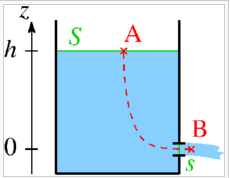
\includegraphics[scale=0.5]{torricelli}
\caption{Formulation du problème de Torricelli}
\label{fig:torricelli}
\end{figure}
En appliquant le théorème de Bernoulli sur une ligne de courant allant de A à B, et en supposant que la vitesse du fluide en A est négligeable, on obtient la formule suivante:
\begin{equation}
v^{2} = 2gh
\end{equation}

\newpage
\bibliographystyle{plain}
\bibliography{biblio}


\end{document} %%% END DOC



























































































